%%%%%%%%%%%%%%%%%%%%%%%%%%%%%%%%%%%%%%%%%%%%%%%
% University Paderborn Beamer Presentation 

% Author: Ashwin Prasad Shivarpatna Venkatesh 

%This template is free: you can redistribute it and/or modify
%it under the terms of the GNU General Public License as published by
%the Free Software Foundation, either version 3 of the License, or any later version.
%
%This program is distributed in the hope that it will be useful,
%but WITHOUT ANY WARRANTY; without even the implied warranty of
%MERCHANTABILITY or FITNESS FOR A PARTICULAR PURPOSE.  See the
%GNU General Public License for more details.
%
%You should have received a copy of the GNU General Public License
%along with this program.  If not, see <https://www.gnu.org/licenses/>.

%%%%%%%%%%%%%%%%%%%%%%%%%%%%%%%%%%%%%%%%%%%%%%%

\documentclass{beamer}
% Default page size 12.8cm x 9.6cm

% import packages and user-defined commands
\usepackage{amsmath, amssymb, amsfonts}% mathematical symbols and the like
\usepackage{amsthm}% definitions, theorems, etc.
\usepackage[colorinlistoftodos]{todonotes}% marking open todos in text/on margins
\usepackage{subfig}% multi-part figures with separate captions per part
\usepackage{url}% render URLs correctly and make them clickable through the hyperref package
\usepackage{longtable}% tables that span multiple pages
\usepackage{booktabs}% tables that actually look good
\usepackage[nolist]{acronym}% consistently use acronyms
\usepackage{caption}
\usepackage{graphicx}
%%%%%%%%%
% Some commands for setting up theorem environments as provided by package 
% amsthm --- language sensitive
%%%%%%%%%
\theoremstyle{plain}
\newtheorem{definition}{Definition}[chapter]
\newtheorem{lemma}[definition]{Lemma}
\ifgerman
	\newtheorem{theorem}[definition]{Satz}
	\newtheorem{corollary}[definition]{Korollar}
	\newtheorem{example}[definition]{Beispiel}
\else
	\newtheorem{theorem}[definition]{Theorem}
	\newtheorem{corollary}[definition]{Corollary}
	\newtheorem{example}[definition]{Example}
\fi


%%%%%%%%%
% Your commands should go here...
%%%%%%%%%
\newcommand*{\eg}{e.\,g.}
\newcommand*{\ie}{i.\,e.}
\newcommand*{\cf}{c.\,f.}
\newcommand*{\etal}{et~al.}

\newcommand{\code}[1]{\texttt{#1}\xspace}

\newacro{template}[UPB-CS-TT]{Paderborn University Computer Science thesis template}

\DeclareMathOperator{\testop}{top}




\definecolor{uni-blue}{cmyk}{1.0, 0.85, 0.05, 0.36, 1.00}
\definecolor{uni-cyan}{cmyk}{0.72, 0.08, 0.0, 0.0, 1.00}
\definecolor{uni-green}{cmyk}{0.50, 0.0, 0.95, 0.0, 1.00}
\definecolor{uni-orange}{cmyk}{0.0, 0.50, 0.95, 0.0, 1.00}
\definecolor{uni-purple}{cmyk}{0.38, 0.88, 0.08, 0.0, 1.00}
\definecolor{uni-gray}{cmyk}{0.0, 0.0, 0.0, 0.30}
\definecolor{uni-black}{cmyk}{0.0, 0.0, 0.0, 0.80}

\setbeamertemplate{navigation symbols}{}
\setbeamercolor{structure}{fg=uni-blue} % itemize, enumerate, etc
\setbeamercolor{normal text}{fg=uni-black}

\setbeamercolor{section in toc}{fg=uni-blue} % TOC sections
\setbeamercolor{subsection in toc}{fg=uni-black} % TOC sections

\setbeamertemplate{subsection  in toc}[square]
\setbeamertemplate{section in toc}[circle]

\setbeamerfont{section number projected}{size=\large}
\setbeamercolor{section number projected}{bg=uni-blue,fg=white}
\setbeamercolor{subsection number projected}{bg=uni-black,fg=white}

% Universal background except title
\usebackgroundtemplate{%
	
\includegraphics[width=\paperwidth,height=\paperheight]{images/otherbackground.pdf}} 

%----------------------------------------------------------------------------------------
%	FOOTER THEME
%----------------------------------------------------------------------------------------

\setbeamertemplate{footline}[text line]{%
		
	\setbeamercolor{footline}{bg=,fg=uni-blue}	
	
	\begin{beamercolorbox}[sep=0.3cm,ht=2.6em,wd=\paperwidth]{footline}
		
		\vbox{}\vskip-2ex%
		\hspace{0.0cm}
		\insertshortauthor
		\hfill
		\fontfamily{phv}\fontseries{bc}\selectfont\bfseries 
		\insertframenumber
		\hfill
		\vskip-0.8ex%
	\end{beamercolorbox}
	
}

%----------------------------------------------------------------------------------------
%	ITEMIZE CIRCLE
%----------------------------------------------------------------------------------------

\setbeamertemplate{itemize items}{
	\begin{tikzpicture}
	\node[circle, draw, semithick, inner sep=0pt, minimum size=4pt] (1) at (0,0) {};
	\end{tikzpicture}
}

%----------------------------------------------------------------------------------------
%	TITLE PAGE
%----------------------------------------------------------------------------------------

\setbeamertemplate{title page}{%

	\begin{tikzpicture}[remember picture,overlay]
	
	% Uni logo
	\node[inner sep=0pt] (logo) at (1.1, 3)
	{
\includegraphics[width=.3\textwidth]{images/logo.pdf}};
	
	% Uni pic
	\node[inner sep=0pt] (logo) at (9.175, 1.62)
	{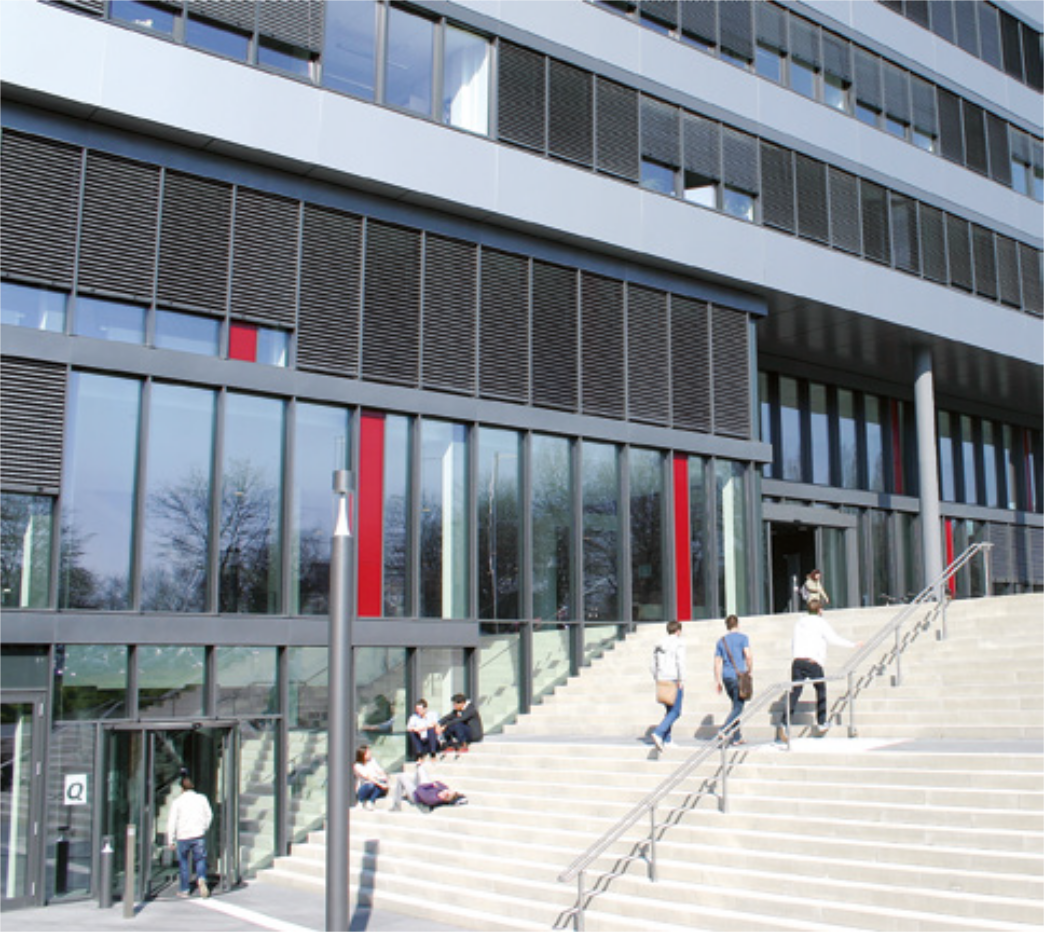
\includegraphics[width=.485\textwidth]{images/unibuilding.png}};
	

	\node[inner sep=0pt] (tit) at (4.40, -2.7)
	{
		\begin{minipage}[t]{1.0\linewidth} 
		\setbeamercolor{title}{bg=\upbcolor,fg=white}	
		
		\begin{minipage}[t]{1.0\linewidth} 
		\setbeamercolor{title}{bg=,fg=uni-blue}	
		\begin{beamercolorbox}[sep=2pt,left]{title}
		{\hspace{4pt}{\vspace{0.1cm}\fontsize{10}{16}\fontfamily{phv}\fontseries{bc}\selectfont\bfseries\insertinstitute}}
		\end{beamercolorbox}
		
		\end{minipage}  	
		
		\begin{minipage}{1.0\linewidth} 
		
		
		\begin{beamercolorbox}[sep=8pt,left]{title}
		
		{\lenitem{\fontsize{\upbtitlesize}{\upbtitlelinespace}\fontfamily{phv}\fontseries{mc}\selectfont\bfseries\color{white}\raggedright\inserttitle}}%
		
		\end{beamercolorbox}
		
		\end{minipage}  	
		
		\ifx\insertsubtitle\@empty%
		\else%
		{		\begin{minipage}[t]{0.9\linewidth} 
			\setbeamercolor{title}{bg=,fg=uni-blue}	
			\begin{beamercolorbox}[sep=4pt,left]{subtitle}
			{\hspace{4pt}\vspace{0.2cm}{\fontsize{10}{16}\fontfamily{phv}\fontseries{bc}\selectfont\bfseries \insertsubtitle}}
			\end{beamercolorbox}
			\end{minipage}  	
		}
		\fi%   			
		
		\end{minipage}  		
		
	};
	
	\end{tikzpicture}	
	
}

%----------------------------------------------------------------------------------------
%	FRAME TITLE THEME
%----------------------------------------------------------------------------------------

\setbeamertemplate{frametitle}
{
	\nointerlineskip
	
	\fontfamily{phv}\fontseries{bc}\selectfont\bfseries 
	\setbeamercolor{frametitle}{bg=,fg=\upbcolor}	
	
	\begin{beamercolorbox}[sep=0.3cm,ht=5.3em,wd=\paperwidth]{frametitle}
		\vbox{}\vskip-2ex%
		\hspace{0.05cm}
		
\includegraphics[width=1.8cm]{images/logo}
		\hfill
		\vskip1.2ex%
		\vspace{0.1cm}
		\hspace{0.0cm}
		\insertframetitle
	\end{beamercolorbox}
	\vspace{-0.4cm}
	
}

% Title
\title{Management of ServiCes Across MultipLE clouds} 

% Sub Title
\subtitle{SCrAMbLE Plug-in Demo}

% Your name
\author{Team PG-SCrambLE}

% Your institution for the title page
\institute{UPB | Computer Networks Group} 

% Date, can be changed to a custom date
\date{\today} 

% Choose primary UPB color for title, headings etc.. 
% Choose from 
% (uni-cyan, uni-black, uni-blue, uni-orange, uni-purple, uni-green)
\newcommand{\upbcolor}{uni-blue} 




%----------------------------------------------------------------------------------------
%	TITLE PAGE
%----------------------------------------------------------------------------------------


\begin{document}

{
\upbtitlebackground 
\begin{frame}
%\upblogo
\titlepage % Print the title page as the first slide
\end{frame}
}

\begin{frame}
\frametitle{Agenda} % Table of contents slide, comment this block out to remove it
\tableofcontents 

\section{Introduction}
\section{Adaptor Demo}
\subsection{Test cases}
\subsection{Front End}
\subsection{MANO Scalability Investigation}
\section{Translator Demo}
\section{Splitter Demo}
\section{Conclusion}



% Throughout your presentation, if you choose to use \section{} and \subsection{} commands, these will automatically be printed on this slide as an overview of your presentation
\end{frame}

%----------------------------------------------------------------------------------------
%	PRESENTATION SLIDES
%----------------------------------------------------------------------------------------
\chapter{Introduction}
\label{ch:Introduction}

\paragraph{ }The aim of technology review is to understand the working of all the tools and technologies relevant for this project.

To achieve this, tasks were assigned to each of the team to review few set of tools as below. 

\begin{figure} [h]
\centering
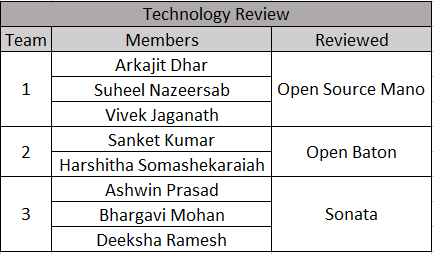
\includegraphics[width=.5\linewidth]{figures/teams}
\end{figure}

MANO frameworks such as Open Source MANO, Sonata and Open Baton have been reviewed in this phase. Different virtual infrastructure managers are tried and worked upon , like Kubernetes and Open Stack.\\*

The MANO frameworks are up and running in virtual machines and the connections are established between MANO and VIM's.\\*

The detailed explanation on installation and steps are given below in the document.




\begin{frame}

\Huge{\centerline{ARCHITECTURE}}

\end{frame}


\begin{frame}

\begin{figure}
	\centering
	
\includegraphics[width=1\linewidth]{images/plugin}
	\label{fig:plugin}
	{\\SCrAMbLE Overview}
\end{figure}


\end{frame}


\begin{frame}
\frametitle{Adaptor Demo}

\Huge{\centerline{Adaptor ---$ > $}}
\end{frame}
\begin{frame}
\frametitle{Adaptor REST API}

\begin{itemize}[<+->]
	\item Unified access to MANO instances			

	\item Implements ETSI endpoints
	\begin{itemize}
		\item Enforce if a MANO is using non-standard endpoint
	\end{itemize}
	
	\item \textbf{MANO}: parameter sent with each request
	\begin{itemize}
		\item Currently supports \textbf{OSM} and \textbf{Sonata}
	\end{itemize}
		
\end{itemize}
\end{frame}

\begin{frame}

\Huge{\centerline{DEMO ---$ > $}}

\end{frame}
\begin{frame}
\frametitle{Test cases}

All the important API calls of OSM and Sonata have been wrapped and test cases for those front end actions are running . . . . 


\Huge{\centerline{DEMO ---$ > $}}
\end{frame}
\begin{frame}
\Huge{\centerline{MANO Scalability Investigation}}
\end{frame}
\begin{frame}
\frametitle{Scalability of a system}

\begin{itemize}
	\item Scaling Approaches
			\begin{itemize}
				\item Service Replication
				\item Proactive and Reactive Scaling
				\item Heirarchical scaling
		\end{itemize}	
	\pause
	\item Scaling effects
	\begin{itemize}
		\item Reliability
		\item Availability 
		\item Heterogeneity
		
	\end{itemize}
	
\end{itemize}

\end{frame}



\begin{frame}

\frametitle{Goals for the coming semester} 

\begin{itemize}
	\item Identify the right approach to scale a MANO taking into account all the effects of scaling
	
	\item Implement ------ ?
	
\end{itemize}


\end{frame}


\begin{frame}

\Huge{\centerline{TRANSLATOR}}
\end{frame}

\begin{frame}
\frametitle{Aim of Translator Service}
\begin{figure}
\centering
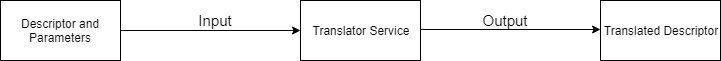
\includegraphics[width=1\linewidth]{images/img-1-translate}
\label{Figure1}
\end{figure}
Translator receives as input descriptor files to be translated and parameters, such as ``Osm-to-Sonata" if OSM descriptor has to be translated to Sonata or ``Sonata-to-osm" if Sonata descriptor has to be translated to OSM. The output of the translator is a translated descriptor as per the parameter 
\end{frame}

\begin{frame}
\frametitle{Working of Translator Service}
\begin{figure}
\centering
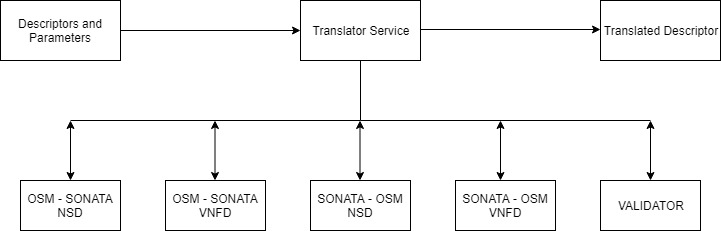
\includegraphics[width=1\linewidth]{images/img-2-translate}
\label{Figure2}
\caption{processing of descriptor file within translator}
\end{figure}
\end{frame}

\begin{frame}
\frametitle{Milestone and challenges}
\textbf{Milestone}:\\
\begin{itemize}
\item The translator can successfully translate simple NSD and VNFD descriptors and validate them.
\end{itemize}

\textbf{Challenges}:\\
\begin{itemize}
\item Translation: have  to work on additional properties such as "monitoring parameters", "forwarding graphs".
\item Validation: Issue with OSM descriptor validation
\end{itemize}

\end{frame}
\begin{frame}
\frametitle{Splitter Demo}
\Huge{\centerline{Splitter}}
\end{frame}


\begin{frame}	
\begin{figure} [!]
	\centering
	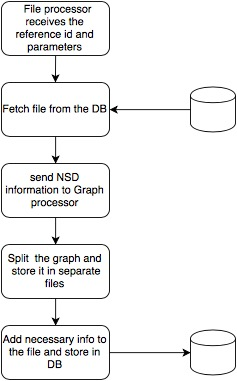
\includegraphics[width=0.3\textwidth]{images/img-1-split}
	\caption{Work-flow of Service Descriptor Splitter}
\end{figure}
\end{frame}

\begin{frame}
\begin{figure}
	\centering 
	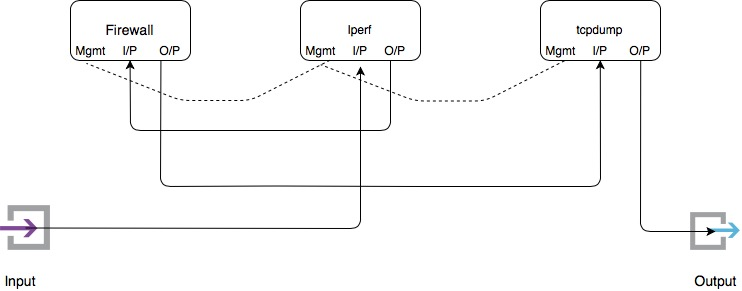
\includegraphics[width=0.5\linewidth]{images/img-2-split}
	\caption{Forwarding-Graph of Sonata NSD}
\end{figure}

\begin{figure}
	\centering 
	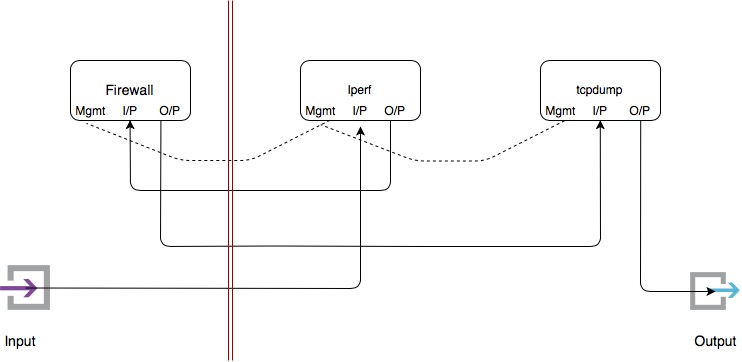
\includegraphics[width=0.5\linewidth]{images/img-3-split}
	\caption{Splitting criteria}
\end{figure}
\end{frame}


\begin{frame}
\begin{figure} 
	\centering
	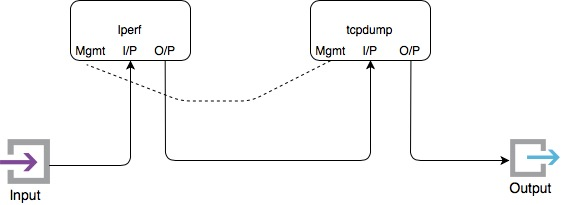
\includegraphics[width=0.6\linewidth]{images/img-4-split}
	\caption{Graph of iperf and tcpdump NSD}
\end{figure}


\begin{figure}
	\centering
	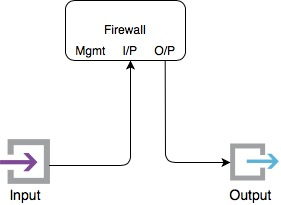
\includegraphics[width=0.3\linewidth]{images/img-5-split}
	\caption{Graph of Firewall NSD}
\end{figure}
\end{frame}



\chapter{Conclusion}
\label{ch:Conclusion}
As discussed previously, there are many challenges to overcome and milestones to be achieved.
At the end, the goal is to build an end product, i.e. OSM adaptor, NSD Splitter and NSD translator but 
an in-depth knowledge on how to achieve it is needed. The next step is to use this document as a base and start reviewing all the technologies and decide upon which ones to use. Design and documention of the architecture which is the foundation to implement the project will begin.
Also in order to be efficient, The project group is divided into sub-groups, to work independently on various topics. Every week the progress of each sub-group is reviewed toshare knowledge and findings to rest of the team. Ultimately, collaborate all the results of the sub-groups to produce a stable end product. 








%------------------------------------------------





%----------------------------------------------------------------------------------------
\begin{frame}
\Huge{\centerline{THE END}}
\end{frame}


\end{document} 